\section{Problem Statement and Model Definition}
\label{sec:mathematical}
To study the spread of news in the population, three types of agents are considered: individuals (also called "people"), \textit{real} news sources, and \textit{fake} news sources. In the context of this research, we define a real news source as a source that spreads reliable, unbiased and fact-checked information. Its opposite, the fake news source, spreads false information. An example of one such network can be seen in Figure~\ref{pics:network_example}.

\begin{figure}
\centering
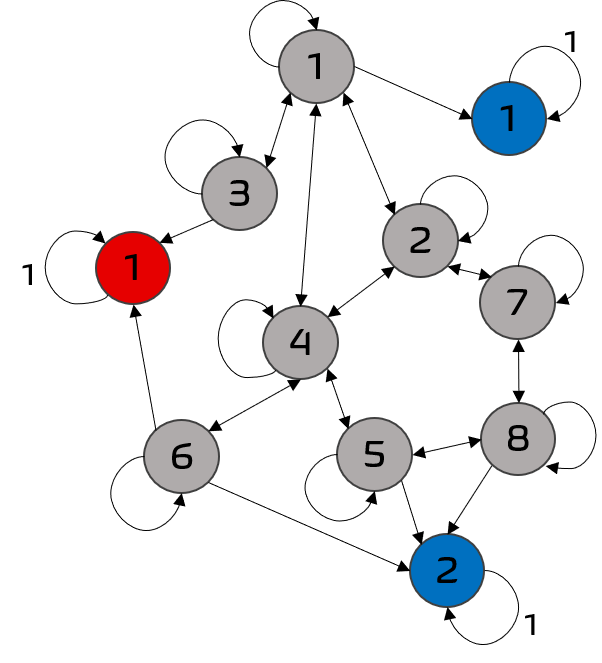
\includegraphics[width=2.5in]{Figures/network_example.png}
\caption{Example of a network that could be generated with our model. The directed graph is formed by eight individuals 1-8, one source of fake news (red), two sources of real news (blue), and links between nodes. Every node has a self loop, with weight 1 for the news sources, and the news sources only have in-neighbors.}
\label{pics:network_example}
\end{figure}
In order to be able to use a multitude of theoretical and analytical tools learned during the course, a linear model with the following update equation is studied
\begin{equation}
\label{eq:model}
x(k+1) = A x(k),
\end{equation}
where $x_i(k) \in [-1;1]$ represents the opinion of individual or source  $i$ at timestep $k$ and $A$ is the adjacency matrix of the network, as in the popular opinion model\cite{Friedkin1990}. Opinion $1$ corresponds to total belief in the real news, while opinion $-1$ corresponds to total belief in the fake news.
Constructing the adjacency matrix $A$ is a non-trivial task as it requires several assumptions on the the existence of links between people, the existence of links between people and news sources, and the importance of each such link.
The existence of links between different individuals and between individuals and sources is determined either by their physical distance or randomly, as will be explained in more detail in Section~\ref{subsec:connections_existence}.
To compute the weights in the adjacency matrix, several qualitative but sensible assumptions are made:

\renewcommand{\theenumi}{\roman{enumi}}
\begin{enumerate}
\item \textit{Similarity}: connections between similar people are stronger. This derives from the fact that people tend to listen to their peers, friends and colleagues more than people that are completely different from them \cite{Youyou2017}\cite{Afifi2013}. Real-world concepts that define similarity may include, but are not limited to: career path, certain behavioral traits, age, nationality, etc.

\item \textit{Influenceability}: different people give different importance to their own personal opinions and can be more or less influenced by external opinions.
\item \textit{Critical thinking}: a person may believe fake or real news sources more or less, depending on how developed their critical thinking ability is.
\end{enumerate}
Mathematically, 
translating these assumptions into a network adjacency matrix $A$ can be done in multiple ways. In this research we mainly present one way that is used for experiments in sections~\ref{sec:Instr_Level} to~\ref{sec:manipulability}, and then a second slightly modified one to investigate opinion polarization in~\ref{sec:polarization}. 

\subsection{Population Matrix}
To build a realistic network, there needs to be some difference between individuals. To differentiate between them, a \textit{population matrix} $B \in \mathbb{R}^{n_p \times t}$ is introduced, where $n_p$ is the number of individuals in the network and $t$ is the number characteristics defined for each person. In this research, $t=3$ and the chosen characteristics are: \textit{similarity}, \textit{influenceability} and \textit{critical thinking ability}. The relative position of an individual inside the matrix $B$ matters, as can be seen in Paragraph~\ref{subsub: connections}. The columns of $B$ are initialized with different random distributions, depending on the desired predominance of traits in the modeled society. Examples of such distributions can be seen in the numerical experiments in Chapter~\ref{sec:experiments}.
\subsection{News Sources}
The number of news sources in the model is an important parameter when creating the network. We define the number of real news sources $n_{r}$ and the number of fake news sources $n_{f}$.
\subsection{Existence of Connections}
\label{subsec:connections_existence}
When generating the adjacency matrix, connections between nodes need to be created.
\subsubsection{Connections Among Individuals}
\label{subsub: connections}
Connections are created based on geographical distance. The real-world is simplified to a straight line with periodic boundaries, where the position of an individual is given by its position inside of the vector $x$. The connection between individuals $i$ and $j$ is created with probability 


\begin{equation}
P(i,j) = \min\left\lbrace 1,\frac{C}{\sqrt[\text{nRoot}]{\vert i-j\vert}}\right\rbrace
\end{equation}
where $C\in \mathbb{R}^*_+$ and nRoot $\in \mathbb{N}^*$ are tunable parameters that shape the probability distribution. $C$ linearly scales the probability of connections between neighbors, while $\text{nRoot}$ defines how quickly $P(i,j)$ decays as a function of $\vert i-j \vert$.

\subsubsection{Connections Among Individuals and Sources}
We define $R$, the \textit{Range}, as the number of connections each news source has, which is given by $R= 10\% (n_p)$, where $n_p$ is the number of individuals.
News connection type is either \textit{local} or \textit{non-local}. 
\\If the news sources are connected locally, for each news source an individual is chosen (uniformly at random) and then this individual and its $R$ geographically closest individuals (on the straight line defined at the beginning of this section) are connected to the news source.
\\If instead the news sources are connected non-locally, $R$ individuals are selected (uniformly at random) and connected to the news source.
\\In our framework, locality and non-locality of news sources can be set independently for real news sources and fake news sources.



\subsection{Importance of Connections}
Once a connection is present, the next step is to define its strength.

\subsubsection{Connections Between Individuals}
If a connection from individual $i$ to individual $j$ exists, the weight $a_{ij}$ is initialized to 1, otherwise to 0 ($a_{ii}$ is always set to 0).
The weights of the connections between individuals $i,j$ are then modified depending on the population matrix $B$. The weights $a_{ij}$ are modified sequentially for each couple of individuals $(i,j)$ according to following three update steps:

\begin{enumerate}
\item[\text{(S1)}] \textit{Similarity:} $a_{ij} \leftarrow \dfrac{a_{ij}}{1 + \vert s_i - s_j\vert}$, with $ i \neq j$ and where $s_i$ is the similarity value of individual $i$. 
\item[\text{(S2)}] \textit{Influenceability:} $a_{ii} \leftarrow \dfrac{10}{1 + f_i}$, where $f_i$ is the influenceability value of individual $i$. The scaling factor $10$ was found empirically by trying to balance the effects of similarity and influenceability on the weights of A, for the baseline cases described in Section~\ref{sec:experiments}.
\end{enumerate}


\subsubsection{Connections Between Individuals and Sources}
\label{subsub:ind_sources}
\begin{enumerate}
\item[\text{(S3)}] \textit{Critical thinking:} the weight of connection from individual $i$ to source $z$ is given by $a_{iz} = k_i$ for real news sources, and $a_{iz} = 1 - k_i$ for fake news sources, where $k_i \in [0,1]$ is the critical thinking parameter of individual $i$. A high critical thinking parameter (close to $1$), will make the individual give a higher importance to true news sources, while a small parameter will give more importance to fake news sources.
\end{enumerate}
After sequentially applying Steps 1-3 as described above, $A$ is normalized along its rows to make it row-stochastic. The matrix $A$ is kept constant for the entire scope of a single experiment.